In einem der Modi soll die Beleuchtung durch den Bewegunsmelder ausgelöst werden. Hierfür sind zuverlässige und weitreichende Bewegungssensoren notwendig.
\subsection{Bewertungskriterien}
\begin{itemize}
\item \textbf{Ansteuerung}\\
Die Anbindung an den Raspberry Pi soll möglichst leicht realisierbar sein. Wünschenswert ist, dass der Sensor einfach ein High-Signal bei Bewegungserkennung ausgibt. \\
Gewichtung: 5, KO-Kriterium
\item \textbf{Reichweite}\\
Die Reichweite oder Sensivität des Sensors soll ausreichend und regelbar sein.\\
Gewichtung: 3
\item \textbf{Kosten}\\
Es werden nur die reinen Produktkosten, also ohne Versand und Zoll, bewertet. \\
Gewichtung: 1
\item \textbf{Extras}\\
An dieser Stelle können mögliche Extras eines Herstellers einfließen.\\
Gewichtung: 3
\end{itemize}

\subsection{Evaluierung}
\begin{itemize}
\item \textbf{PIR (MOTION) Sensor, Adafruit}\\
Link: http://www.adafruit.com/product/189\\
Ansteuerung: Gibt High-Signal an einem Pin aus.\\
Reichweite: 7m, 120 Grad\\
Kosten: 9,95\$ + Versand aus USA\\
Extras: Kabel inklusive\\
\item \textbf{PIR Infrared Motion Sensor (HC-SR501)}\\
Link: https://www.modmypi.com/pir-motion-sensor\\
Ansteuerung: Gibt High-Signal an einem Pin aus.\\
Reichweite: 5-7m, 100 Grad\\
Kosten: 2,99\$ + Versand aus UK\\
Extras: keine\\
\item \textbf{Infrarot PIR Bewegung Sensor Detektor Modul}\\
Link: http://www.amazon.de/Pyroelectrische-Infrarot-Bewegung-Sensor-Detektor/dp/B008AESDSY/ref=pd\_cp\_ce\_0\\
Ansteuerung: Gibt High-Signal an einem Pin aus.\\
Reichweite: 7m, 100 Grad\\
Kosten: 5 Stück = 7,66€\\
Extras: keine\\
\end{itemize}
\begin{minipage}{\linewidth}
            \centering
            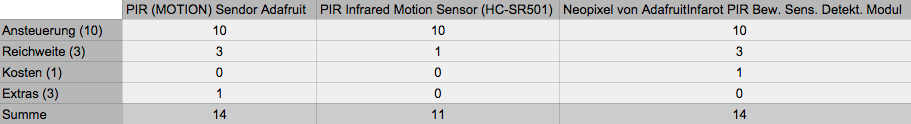
\includegraphics[width=\textwidth]{./data/evaluierung-ms.png}
            \captionof{figure}{Ergebnisse der Motion-Sensor-Evaluierung}
        \end{minipage}
\paragraph{Fazit}
Die meisten Infarot-Bewegungssensoren sind von der Bauweise nahezu identisch. Die Unterschiede liegen meist nur in der Empfindlichkeit. Da die Reichweite in diesem Fall nicht von großer Bedeutsamkeit ist, kann eigentlich jedes der Produkte bestellt werden. Auf Ebay und Amazon ist die Anzahl angebotener Sensoren nahezu unbegrenzt, es wurde für die Teststellung also die oben evaluierte Variante von Amazon bestellt. 
\subsection{Teststellung}
Der in Punkt X.X.X gewählte Bewegungssensor wurde beim Hersteller bestellt. In der Teststellung reicht die Stromversorgung des Raspberry Pi. 
\paragraph{Technische Daten Sensor:}
\begin{itemize}
\item Die Empfindlichkeit und Haltezeit kann eingestellt werden
\item Reichweite: ca. 7m
\item Winkel: 100 Grad
\item Spannung: DC 4,5V- 20V
\item Strom: < 50uA
\item Ausgansspannung: High 3V / Low 0V
\item Größe: ca. 32mm x 24mm
\end{itemize}

\paragraph{Ablauf des Tests:}
\begin{itemize}
\item \textbf{Aufbau der Schaltung} \\
Der Sensor wird in der Teststellung direkt vom Raspberry Pi mit Strom versorgt. Für die Datenleitung kann jeder beliebige Pin gewählt werden. 
\item \textbf{Testcode} \\
Um eine Änderung am Datenpin festzustellen werden zwei Variable angelegt: current\_status und previous\_status. Das Programm wird in einer Dauerschleife geschickt, in der bei jedem Durchlauf die beiden Status überprüft. Wenn der neue Status (current\_status) High ist und das vorherige Signal (previous\_state) Low, dann wird eine Bewegung erkannt. Der Code wird mittels Kommentare erklärt.	

\begin{lstlisting}[caption = Testcode zur Bewegungserkennung mit Sensor, language=python, frame=single, breaklines=true,columns=fullflexible, commentstyle=\color{gray}\upshape, captionpos=b, numbers = left]
import RPi.GPIO as GPIO
import time

GPIO.setmode(GPIO.BCM)
	
# Pin definieren
MOTION_PIN1 = 7
	
# Diese als Input definieren
GPIO.setup(MOTION_PIN1,GPIO.IN)

# Status definieren um verschiedene Änderungen zu erkennen
Current_State  = 0
Previous_State = 0
					
try:
	# Loop zur Erkennung einer Bewegung
	# Sensor erkennt Bewegung -> Signal = High
	# Wartet 3 Sekunden und setzt Signal = Low
	while True :
		Current_State = GPIO.input(MOTION_PIN1)
		if Current_State == 1 and Previous_State == 0:
			print "Motion detected!"
			Previous_State=1
		elif Current_State == 0 and Previous_State == 1:
			print "Ready"
			Previous_State=0
		time.sleep(0.01)
	
except KeyboardInterrupt:
	print "Quit"
	GPIO.cleanup()
\end{lstlisting}
Bei der Endversion des Systems sollen mehrere Beweungssensoren integriert werden. Bei Auslösen des ersten Sensors sollen die LEDs angeschaltet werden und nach auslösen eines weiteren Sensors wieder ausgeschaltet werden. 
\paragraph{Auswertung}\\
Das High-Signal des Sensors lässt sich mit dem Raspberry Pi sehr leicht auswerten. Auch die Auswertung von mehreren Sensoren stellt kein Problem da. Das Ergebnis der Evaluierung konnte in dieser Tststellung bestätigt werden. 
\end{itemize}
